    \documentclass[oneside,a4paper,14pt]{extarticle} %размер шрифта 14
\usepackage[T1,T2A]{fontenc}
\usepackage[a4paper,% размер страницы
letterpaper,top=20mm,bottom=20mm,
left=30mm,right=10mm]{geometry} %размеры пустых полей
% Можно так \usepackage[left=2.5cm,right=1.5cm,top=2cm,bottom=2cm]
%{geometry} 
\usepackage[utf8]{inputenc} %кодировка текста
\usepackage[russian]{babel} %поддержка русского языка
\usepackage{textcomp} %текстовые символы
\usepackage{indentfirst} %корректировка отступов
\usepackage{graphicx} %работа с изображениям
\usepackage{mwe} % for blindtext and example-image-a in example
\usepackage{wrapfig}
\usepackage{caption}
\usepackage{amsmath}  % для формул и символов
\usepackage{amsfonts}
\usepackage{amsthm}
\usepackage{graphicx}
\usepackage[all]{xy}
\usepackage[breaklinks]{hyperref} %размеркегляузаголоковразделов 
\usepackage{titlesec} 
\usepackage{listings}
\usepackage{verbatim, fancyvrb} % Листинг
\usepackage{minted, fancyvrb} % Листинг

% Форматирование листингов с кодом
\setminted{style = rainbow_dash, fontsize = \small}

% Форматирование заголовков
\titleformat{\section}{\normalsize\bfseries}{\thesection}{1em}{}
\titleformat{\subsection}{\normalsize\bfseries}{\thesubsection}{1em}{}
\titleformat{\subsubsection}{\normalsize\bfseries}{\thesubsubsection}{1em}{}

\titleformat{\section}
{\normalsize\bfseries} 
{\thesection} {1em}{} 
\titleformat{\subsection}
{\normalsize\bfseries}
{\thesubsection} {1em}{} 
\titleformat{\subsubsection}
{\normalsize\bfseries}
{\thesubsection} {1em}{}

\renewcommand\baselinestretch{1.33}\normalsize % межстрочный интервал
\setlength{\parindent}{1.25cm}
\usepackage{indentfirst}


\begin{document}
\newpage\thispagestyle{empty}
\begin{center}
	МИНИСТЕРСТВО НАУКИ И ВЫСШЕГО ОБРАЗОВАНИЯ\\
	РОССИЙСКОЙ ФЕДЕРАЦИИ
	ФЕДЕРАЛЬНОЕ ГОСУДАРСТВЕННОЕ БЮДЖЕТНОЕ\\
	ОБРАЗОВАТЕЛЬНОЕ
	УЧРЕЖДЕНИЕ ВЫСШЕГО ОБРАЗОВАНИЯ\\
	«ВЯТСКИЙ ГОСУДАРСТВЕННЫЙ УНИВЕРСИТЕТ»\\
	Институт математики и информационных систем\\
	Факультет автоматики и вычислительной техники\\
	Кафедра электронных вычислительных машин
\end{center}
\vspace{30mm}

\begin{center}
	Отчёт по лабораторной работе №2\\
	по дисциплине\\
	<<Введение в аппаратное обеспечение систем искусственного интеллекта>>\\

\end{center}
\vspace{40mm}

\noindent
\begin{tabular}{l r}

	Выполнил студент гр. ИВТб-1303-06-00
	\hspace{15mm} \rule[-1mm]{30mm}{0.15mm}\,/Шубин В.Ю./ \\ % Своё ФИО


	Проверил доцент кафедры ЭВМ \hfill
	\rule[-1mm]{30mm}{0.15mm}\,/Коржавина А.С./
\end{tabular}

\vfill
\begin{center}
	Киров\\
	2026
\end{center}



\newpage\thispagestyle{empty}


\section{Задания:}
    
    \subsection[short]{Секундомер с драйвером 4026}
    \textbf{Цель:} Собрать секундомер с драйвером 4026, считающий числа заданной последовательности.\\
    \textbf{Вариант:} 3\\
    \textbf{Последовательность:} \href{https://oeis.org/search?q=A006995&language=english&go=Search}{Двоично-десятичные палиндромы (A006995)}\\
    \textbf{Сборка (общ.):} Счетчик нажатий\\
      
    \begin{flushleft}
    \begin{figure}[h!]
        \centering
        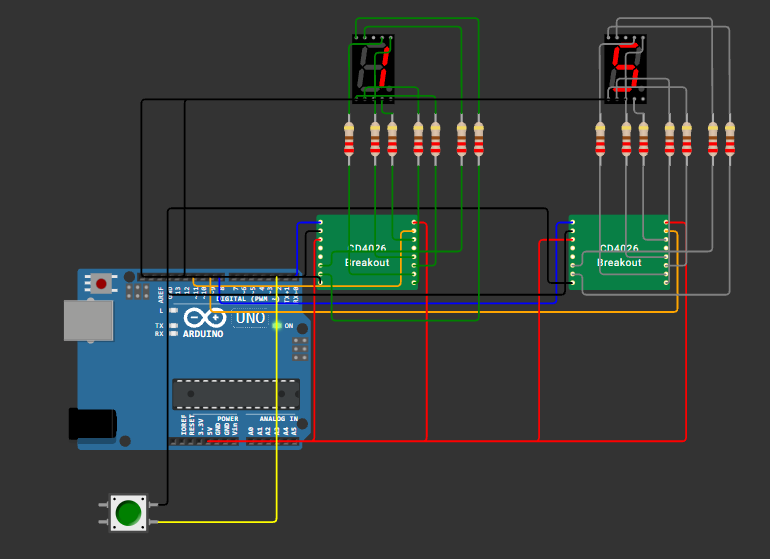
\includegraphics[width=0.85\textwidth]{4026.png}  
        \caption*{Секундомер с драйвером 4026 - сборка}
    \end{figure}
    \end{flushleft}

    \newpage
    Исходный код:
    \inputminted[fontsize=\fontsize{10pt}{13pt}]{c}{4026.c}

    % \newpage
    % \begin{flushleft}
    % \begin{figure}[h!]
    %     \centering
    %     \includegraphics[width=1.0\textwidth]{}  
    %     \caption*{Секундомер с драйвером 4026 - схема}
    % \end{figure}
    % \end{flushleft}

    Ссылка на сборку: https://wokwi.com/projects/481404027439578113




    \newpage
    \subsection[short]{Секундомер на микросхеме К176ИЕ4}
    \textbf{Цель:} Собрать секундомер на микросхеме К176ИЕ4, считающий числа заданной последовательности.\\
    \textbf{Вариант:} 3\\
    \textbf{Последовательность:} \href{https://oeis.org/search?q=A006995&language=english&go=Search}{Двоично-десятичные палиндромы (A006995)}\\
    \textbf{Сборка (общ.):} катод\\
      
    \begin{flushleft}
    \begin{figure}[h!]
        \centering
        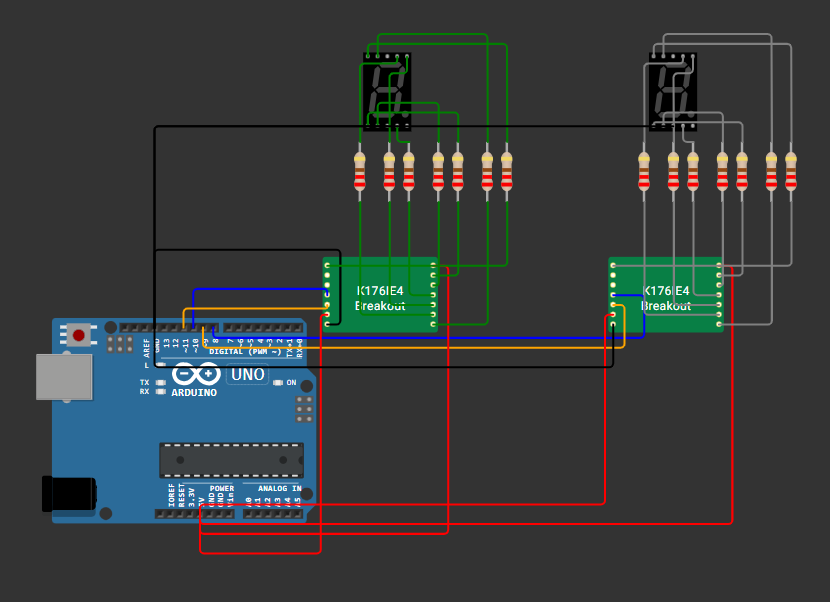
\includegraphics[width=0.85\textwidth]{к176ие4.png}  
        \caption*{Секундомер на микросхеме К176ИЕ4 - сборка}
    \end{figure}
    \end{flushleft}

    \newpage
    Исходный код:
    \inputminted{c}{k176.c}

    % \newpage
    % \begin{flushleft}
    % \begin{figure}[h!]
    %     \centering
    %     \includegraphics[width=1.0\textwidth]{}  
    %     \caption*{Секундомер на микросхеме К176ИЕ4 - схема}
    % \end{figure}
    % \end{flushleft}

    Ссылка на сборку: https://wokwi.com/projects/481403934802042881





    \newpage
    \subsection[short]{Светодиодная матрица 8x8 (Troyka модуль)}
    \textbf{Цель:} Отобразить на матрице изменение состояний.\\
    \textbf{Вариант:} 3\\
      
    \begin{flushleft}
    \begin{figure}[h!]
        \centering
        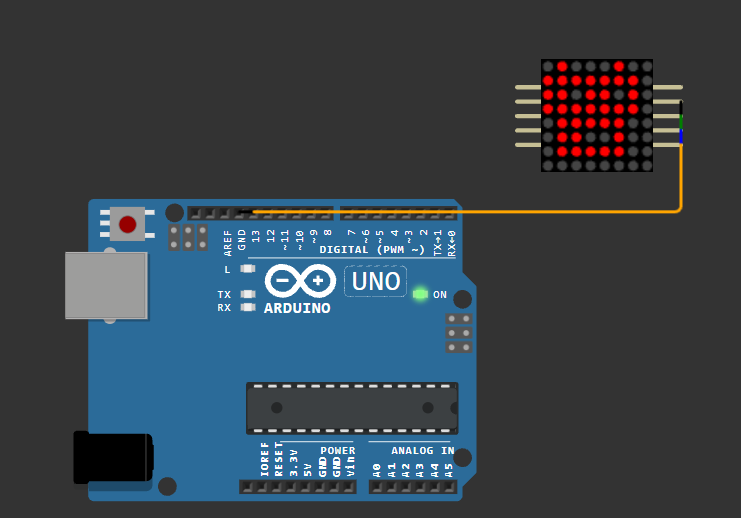
\includegraphics[width=0.85\textwidth]{матрица.png}  
        \caption*{Светодиодная матрица 8x8 - сборка}
    \end{figure}
    \end{flushleft}

    \newpage
    Исходный код:
    \inputminted{c}{matrix.c}

    % \newpage
    % \begin{flushleft}
    % \begin{figure}[h!]
    %     \centering
    %     \includegraphics[width=1.0\textwidth]{}  
    %     \caption*{Светодиодная матрица 8x8 - схема}
    % \end{figure}
    % \end{flushleft}

    Ссылка на сборку: https://wokwi.com/projects/481403926577008641

\newpage
\section*{Вывод:}
В ходе выполнения лабораторной работы на практике закрепил навыки управления семисегментными индикаторами с помощью микросхем-драйверов и светодиодной матрицей. Для варианта 3 была реализована выдача членов последовательности двоично-десятичных палиндромов (A006995) на индикаторах 4026 и К176ИЕ4, а также анимация трёх состояний на матрице 8x8.
% Меняем в каждой лабораторной работе. Ориентируемся на Цель
\end{document}
